\PassOptionsToPackage{dvipsnames}{xcolor}
\documentclass[10pt, oneside]{article}   	% use "amsart" instead of "article" for AMSLaTeX format
\usepackage{geometry}                		% See geometry.pdf to learn the layout options. There are lots.
\geometry{letterpaper}                   		% ... or a4paper or a5paper or ... 
%\geometry{landscape}                		% Activate for rotated page geometry
%\usepackage[parfill]{parskip}    		% Activate to begin paragraphs with an empty line rather than an indent
\usepackage{graphicx}				% Use pdf, png, jpg, or eps§ with pdflatex; use eps in DVI mode
								% TeX will automatically convert eps --> pdf in pdflatex		
\usepackage{setspace}
\setstretch{0.5}

\usepackage{lmodern}
\usepackage{amsmath,amssymb,amsthm,enumitem,mathtools,xpatch}
\usepackage{bm}
\usepackage[most]{tcolorbox}
\usepackage[dvipsnames]{xcolor}
\newcommand*{\simsym}{\mathord\sim}\usepackage{amsthm}
\usepackage{float}
\usepackage{mathrsfs}
\usepackage{wrapfig, lipsum, amsthm, thmtools}
\usepackage{geometry}
 \geometry{
 a4paper,
 total={170mm,257mm},
 left=15mm,
 right = 15mm,
 top=15mm,
 bottom = 20mm
 }


\newcommand*{\Perm}[2]{{}^{#1}\!P_{#2}}%
\newcommand*{\Comb}[2]{{}^{#1}C_{#2}}%

\usepackage[framemethod=tikz]{mdframed}

\theoremstyle{definition}
\newtheorem*{exmp*}{Example}

\newtheorem*{defn}{Definition}
\surroundwithmdframed[backgroundcolor=white]{defn}

\newtheorem{cor}{Corollary}
\surroundwithmdframed[backgroundcolor=white]{cor}

\newtheorem{prop}{Proposition}
\surroundwithmdframed[backgroundcolor=white]{prop}

\newtheorem*{thm}{Theorem}
\surroundwithmdframed[backgroundcolor=white]{thm}


% tikz for probability tree

\usepackage[latin1]{inputenc}
\usepackage{tikz}
\usetikzlibrary{trees,calc,angles,positioning,intersections}

% pgfplot

\usepackage{pgfplots}
\pgfplotsset{width=10cm,compat=1.9}

% quotations dirty talk
\usepackage{dirtytalk}

% floor ceiling
\DeclarePairedDelimiter\ceil{\lceil}{\rceil}
\DeclarePairedDelimiter\floor{\lfloor}{\rfloor}


\title{Introductory Probability and Statistical Applications, Second Edition \\
\large{Paul L. Meyer}}
\author{Notes and Solutions by David A. Lee}
\date{}							% Activate to display a given date or no date

\begin{document}
\maketitle
\section*{Solutions to Chapter 4: One-Dimensional Random Variables}

Unfinished problems: 4.23(a)(b), 4.26(a), 4.27(b)

\begin{enumerate}[label=4.\arabic*]
\itemsep0em 
%Question 4.1
\item  \begin{tcolorbox}[
  colback=Cerulean!5!white,
  colframe=Cerulean!75!black]
\textbf{A coin is known to come up heads three times as often as tails. This coin is tossed three times. Let $\bm{X}$ be the number of heads that appear. Write out the probability distribution of $\bm{X}$ and also the cdf. Make a sketch of both.}
\end{tcolorbox}

We have $X = \{0, 1, 2, 3 \}$. By premise, $P(H) = 3/4, P(T) = 1/4$. The sample space is 

\[ \{ HHH, HHT, HTH, THH, HTT, THT, TTH, TTT \} \] 

It follows that $P(X = 0) = 1/64, P(X = 1) = 9/64, P(X = 2) = 27/64, P(X = 3) = 27/64$. The corresponding cdf is $P(X \leq 0) = 1/64, P(X \leq 1) = 10/64, P(X \leq 2) = 37/64, P(X \leq 3) = 1$. Alternatively, since this is a binomial distribution, $P(X = 0) = \binom{3}{0}(3/4)^0 (1/4)^3 = 1/64, P(X = 1) = \binom{3}{1}(3/4)^1 (1/4)^2 = 9/64, P(X = 2) = \binom{3}{2}(3/4)^2 (1/4)^1 = 27/64, P(X = 3) = \binom{3}{3}(3/4)^3 (1/4)^0 = 27/64$. Graphically,

\begin{center}
\begin{tikzpicture}[scale=0.75]
	\begin{axis}
	[% 
	scatter/classes={%
		a={mark=square*,blue},%
		b={mark=triangle*,red},%
		c={mark=o,draw=black}},
		xlabel={$X$},
		ylabel={$P(X)$},
		xtick={0, 1, 2, 3},
		ytick={0.25, 0.5, 0.75, 1},
		ymax=1]
	\addplot[scatter,only marks,%
		scatter src=explicit symbolic]%
	table[meta=label] {
x     y      label
0      0.0156   a     
1      0.1406   a     
2      0.4219   a
3      0.4219   a     
	};
	\end{axis}
	\node[align=center,font=\bfseries, xshift=1.5em, yshift=1em] (title) 
    at (current bounding box.north)
    {Probability Distribution};
\end{tikzpicture}
\begin{tikzpicture}[scale=0.75]
	\begin{axis}
	[% 
	scatter/classes={%
		a={mark=square*,blue},%
		b={mark=triangle*,red},%
		c={mark=o,draw=black}},
		xlabel={$X$},
		ylabel={$P(X)$},
		xtick={0, 1, 2, 3},
		ytick={0.25, 0.5, 0.75, 1},
		ymax=1]
	\addplot[scatter,only marks,%
		scatter src=explicit symbolic]%
	table[meta=label] {
x     y      label
0      0.0156   a     
1      0.1562   a     
2      0.5781   a
3      1   a     
	};
	\end{axis}
		\node[align=center,font=\bfseries, xshift=1.5em, yshift=1em] (title) 
    at (current bounding box.north)
    {Cumulative Distribution Function};
\end{tikzpicture}
\end{center}

%Question 4.2
\item  \begin{tcolorbox}[
  colback=Cerulean!5!white,
  colframe=Cerulean!75!black]
\textbf{From a lot containing 25 items, 5 of which are defective, 4 are chosen at random. Let $\bm{X}$ be the number of defectives found. Obtain the probability distribution of $\bm{X}$ if}
\end{tcolorbox}

Let $X$ be the number of defectives found in a set of four. We have $\{ X = 0, 1, 2, 3, 4\}$. Then the sample space is (for $D = $ defective and $N =$ normal)
	
\begin{align*}
\{ NNNN, DNNN, NDNN, NNDN, NNND, DDNN, NDDN, NNDD, DNDN, \\
NDND, DNND, DDDN, NDDD, DDND, DNDD, DDDD \}
\end{align*}

	\begin{enumerate}
	%Question 4.2(a)
	\item  \begin{tcolorbox}[
	  colback=Cerulean!5!white,
	  colframe=Cerulean!75!black]
	\textbf{the items are chosen with replacement,}
	\end{tcolorbox}
	
	\begin{align*}
	P(X = 0) &= (4/5)^4 = 0.4096 \\
	P(X = 1) &=  4 \cdot (4/5)^3 (1/5) = 0.4096 \\
	P(X = 2) &= 6 \cdot (4/5)^2 (1/5)^2 = 0.1536 \\
	P(X = 3) &= 4 \cdot (4/5) (1/5)^3 = 0.0256 \\
	P(X = 4) &= (1/5)^4 = 0.0016
	\end{align*}
	
	Equivalently, since this is a binomial distribution, use $P(X = k) = \binom{4}{k} (1/5)^k (4/5)^{n-k}$ for $k = 0, ..., 4$.
	
	\begin{center}
\begin{tikzpicture}[scale=0.75]
	\begin{axis}
	[% 
	scatter/classes={%
		a={mark=square*,blue},%
		b={mark=triangle*,red},%
		c={mark=o,draw=black}},
		xlabel={$X$},
		ylabel={$P(X)$},
		xtick={0, 1, 2, 3, 4},
		ytick={0.25, 0.5, 0.75, 1},
		ymax=1]
	\addplot[scatter,only marks,%
		scatter src=explicit symbolic]%
	table[meta=label] {
x     y      label
0      0.4096   a     
1      0.4096   a     
2      0.1536   a
3      0.0256   a     
4	0.0016  a
	};
	\end{axis}
	\node[align=center,font=\bfseries, xshift=1.5em, yshift=1em] (title) 
    at (current bounding box.north)
    {Probability Distribution};
\end{tikzpicture}
\begin{tikzpicture}[scale=0.75]
	\begin{axis}
	[% 
	scatter/classes={%
		a={mark=square*,blue},%
		b={mark=triangle*,red},%
		c={mark=o,draw=black}},
		xlabel={$X$},
		ylabel={$P(X)$},
		xtick={0, 1, 2, 3, 4},
		ytick={0.25, 0.5, 0.75, 1},
		ymax=1]
	\addplot[scatter,only marks,%
		scatter src=explicit symbolic]%
	table[meta=label] {
x     y      label
0      0.4096   a     
1	0.8192  a
2      0.9728   a     
3      0.9984   a
4      1   a   	  
	};
	\end{axis}
		\node[align=center,font=\bfseries, xshift=1.5em, yshift=1em] (title) 
    at (current bounding box.north)
    {Cumulative Distribution Function};
\end{tikzpicture}
\end{center}
	
	%Question 4.2(b)
	\item  \begin{tcolorbox}[
	  colback=Cerulean!5!white,
	  colframe=Cerulean!75!black]
	\textbf{the items are chosen without replacement.}
	\end{tcolorbox}
	
	Critically, note that this is not a binomial distribution as each of the four successive drawings are \textbf{not} independent of one another. Then we calculate the probability of each outcome of $X$ as
	
	\begin{align*}
	P(X = 0) &= (20/25)(19/24)(18/23)(17/22) = 0.3830 \\
	P(X = 1) &= 4 \cdot (5/25)(20/24)(19/23)(18/22) = 0.4506 \\
	P(X = 2) &= 6 \cdot (5/25)(4/24)(20/23)(19/22) = 0.1502 \\
	P(X = 3) &= 4 \cdot (5/25)(4/24)(3/23)(20/22) = 0.0158 \\
	P(X = 4) &= (5/25)(4/24)(3/23)(2/22) = 0.0004
	\end{align*}
	
	Alternatively, observe that \textbf{with} replacement, the distribution is binomial, and \textbf{without}, it becomes hypergeometric. Then for any value of $X$, we can use the hypergeometric probability $\binom{5}{x} \binom{20}{4 - x} / \binom{25}{4}$.
	
		\begin{center}
\begin{tikzpicture}[scale=0.75]
	\begin{axis}
	[% 
	scatter/classes={%
		a={mark=square*,blue},%
		b={mark=triangle*,red},%
		c={mark=o,draw=black}},
		xlabel={$X$},
		ylabel={$P(X)$},
		xtick={0, 1, 2, 3, 4},
		ytick={0.25, 0.5, 0.75, 1},
		ymax=1]
	\addplot[scatter,only marks,%
		scatter src=explicit symbolic]%
	table[meta=label] {
x     y      label
0      0.3830   a     
1      0.4506   a     
2      0.1502   a
3      0.0158   a     
4	0.0004  a
	};
	\end{axis}
	\node[align=center,font=\bfseries, xshift=1.5em, yshift=1em] (title) 
    at (current bounding box.north)
    {Probability Distribution};
\end{tikzpicture}
\begin{tikzpicture}[scale=0.75]
	\begin{axis}
	[% 
	scatter/classes={%
		a={mark=square*,blue},%
		b={mark=triangle*,red},%
		c={mark=o,draw=black}},
		xlabel={$X$},
		ylabel={$P(X)$},
		xtick={0, 1, 2, 3, 4},
		ytick={0.25, 0.5, 0.75, 1},
		ymax=1]
	\addplot[scatter,only marks,%
		scatter src=explicit symbolic]%
	table[meta=label] {
x     y      label
0      0.3830   a     
1	0.8336  a
2      0.9838   a     
3      0.9996   a
4      1   a   	  
	};
	\end{axis}
		\node[align=center,font=\bfseries, xshift=1.5em, yshift=1em] (title) 
    at (current bounding box.north)
    {Cumulative Distribution Function};
\end{tikzpicture}
\end{center}
	\end{enumerate}

%Question 4.3
\item  \begin{tcolorbox}[
  colback=Cerulean!5!white,
  colframe=Cerulean!75!black]
\textbf{Suppose that the random variable $\bm{X}$ has possible values 1, 2, 3, ..., and $\bm{P(X = j) = 1/2^j, j = 1, 2, ...}$}
\end{tcolorbox}

	\begin{enumerate}
	%Question 4.3(a)
	\item  \begin{tcolorbox}[
	  colback=Cerulean!5!white,
	  colframe=Cerulean!75!black]
	\textbf{Compute $\bm{P(X \text{ is even})}$.}
	\end{tcolorbox}
	
	Observe that we derive the geometric series $P(X \text{ is even}) = \sum^\infty_{j = 2, 2 | j} 1/2^j = 1/4 + 1/16 + 1/64 + \cdots = \frac{1/4}{1 - 1/4} = \boxed{1/3}$.
	
	%Question 4.3(b)
	\item  \begin{tcolorbox}[
	  colback=Cerulean!5!white,
	  colframe=Cerulean!75!black]
	\textbf{Compute $\bm{P(X \geq 5)}$.}
	\end{tcolorbox}
	
	$\sum^\infty_{j = 1} 1/2^j - \sum^{4}_{j = 1} 1/2^j = \frac{1/2}{1 - 1/2} - (1/2 + 1/4 + 1/8 + 1/16) = \boxed{1/16}$.
	
	%Question 4.3(c)
	\item  \begin{tcolorbox}[
	  colback=Cerulean!5!white,
	  colframe=Cerulean!75!black]
	\textbf{Compute $\bm{P(X \text{ is divisible by }3)}$.}
	\end{tcolorbox}
	
	$\sum^\infty_{j = 3, 3 | j} 1/2^j = 1/8 + 1/64 + \cdots = \frac{1/8}{1 - 1/8} = \boxed{1/7}.$
	\end{enumerate}
	
%Question 4.4
\item  \begin{tcolorbox}[
  colback=Cerulean!5!white,
  colframe=Cerulean!75!black]
\textbf{Consider a random variable $\bm{X}$ with possible outcomes: 0, 1, 2, ... Suppose that $\bm{P(X = j) = (1 - a)a^j, j = 0, 1, 2, ...}$}
\end{tcolorbox}

	\begin{enumerate}
	%Question 4.4(a)
	\item  \begin{tcolorbox}[
	  colback=Cerulean!5!white,
	  colframe=Cerulean!75!black]
	\textbf{For what values of $\bm{a}$ is the above model meaningful?}
	\end{tcolorbox}
	
	By definition, a probability $p$ must be bounded by $0 \leq p \leq 1$, and this condition fails for $a < 0$ and $a > 1$. Therefore, we must have $0 \leq a \leq 1$. Really, we should be stricter and require $0 < a < 1$ as $P(X = j)$ vanishes otherwise.
	
	%Question 4.4(b)
	\item  \begin{tcolorbox}[
	  colback=Cerulean!5!white,
	  colframe=Cerulean!75!black]
	\textbf{Verify that the above does represent a legitimate probability distribution.}
	\end{tcolorbox}
	
	Satisfying Meyer Definition 1.3:
	
	\textbf{(1)} For $0 < a < 1$, $0 < (1 - a)a^j < 1 \ \forall j$. This is true for $j = 0$, as $0 < 1-a < 1$. Suppose it is true for $j = 1, ..., n-1$. Then it follows that $0 < (1 - a)a^n < (1-a)a^{n-1} < 1$. Therefore $0 < P(X = j) < 1$.
	
	\textbf{(2)} The sample space $S$ is choosing zero or any natural number. It follows that $P(S) = \sum^\infty_{j = 0} = (1 - a)a^j = (1-a) \frac{1}{1-a} = 1$.
	
	\textbf{(3)} For any arbitrary $j_i$ or $j_k$, $X = j_i$ and $X = j_k$ are mutually exclusive, for $X$ can only take on one value. Then $P(X = j_i \text{ or } X = j_k) = (1 - a)a^{j_i} + (1 - a)a^{j_k} = (1 - a)(a^{j_i} + a^{j_k})$.
	
	\textbf{(4)} See (2).
	
	%Question 4.4(c)
	\item  \begin{tcolorbox}[
	  colback=Cerulean!5!white,
	  colframe=Cerulean!75!black]
	\textbf{Show that for any two positive integers $\bm{s}$ and $\bm{t}$, $\bm{P(X > s + t | X > s) = P(X \geq t)}$.}
	\end{tcolorbox}
	
	\begin{proof}
	By definition of conditional probability:
	
	\begin{align*}
	P(X > s + t | X > s) &= \frac{P(X > s + t)}{P(X > s)} \\
	&= \frac{\sum^\infty_{j = s + t + 1} (1-a)a^j}{\sum^\infty_{j = s + 1} (1-a)a^j} \\
	&= \frac{\sum^\infty_{j = 0} (1-a)a^j - \sum^{s+t}_{j = 0} (1-a)a^j}{\sum^\infty_{j = 0} (1-a)a^j - \sum^{s}_{j = 0} (1-a)a^j} \\
	&= \frac{1 - (1 - a^{s+t+1} ) }{1 - ( 1 - a^{s+1} ) } \\
	&= \frac{a^{s+t+1} }{a^{s+1} } \\
	&= a^t \\
	&= 1 - \Bigg( \frac{1 - a^t}{1-a} \Bigg) (1-a) \\
	&= \sum^\infty_{j = t} (1-a)a^j = P(X \geq t)
	\end{align*}
	\end{proof}
	\end{enumerate}
	
%Question 4.5
\item  \begin{tcolorbox}[
  colback=Cerulean!5!white,
  colframe=Cerulean!75!black]
\textbf{Suppose that twice as many items are produced (per day) by machine 1 as by machine 2. However, about 4 percent of the items from machine 1 tend to be defective while machine 2 produces only about 2 percent defectives. Suppose that the daily output of the two machines is combined. A random sample of 10 is taken from the combined output. What is the probability that this sample contains 2 defectives?}
\end{tcolorbox}

By premise, $P(M1) = 2/3$ and $P(M2) = 1/3$. Moreover, $P(D | M1) = 0.04$ and $P(D | M2) = 0.02$. By the law of total probability, $P(D) = P(D | M1) P(M1) + P(D | M2) P(M2) = (0.04)(2/3) + (0.02)(1/3) = 1/30$. Suppose that $n$ items are collectively produced by the two machines. Let $k = n/30$ be the number of defective items. Then the probability of finding 2 defectives in a sample of 10 is $\boxed{ \binom{k}{2} \binom{n-k}{8} / \binom{n}{10} }$.

%Question 4.6
\item  \begin{tcolorbox}[
  colback=Cerulean!5!white,
  colframe=Cerulean!75!black]
\textbf{Rockets are launched until the first successful launching has taken place. If this does not occur within 5 attempts, the experiment is halted and the equipment inspected. Suppose that there is a constant probability of 0.8 of having a successful launching and that successive attempts are independent. Assume that the cost of the first launching is $\bm{K}$ dollars while subsequent launchings cost $\bm{K/3}$ dollars. Whenever a successful launching takes place, a certain amount of information is obtained which may be expressed as financial gain of, say $\bm{C}$ dollars. If $\bm{T}$ is the net cost of this experiment, find the probability distribution of $\bm{T}$.}
\end{tcolorbox}

By independence of each successive launch, if $X$ is the $i$-th launch that the rocket successfully launches, we have

\begin{align*}
P(X = 1) &= 0.8 \\
P(X = 2) &= (0.2)(0.8) = 0.16 \\
P(X = 3) &= (0.2)^2 (0.8) = 0.032 \\
P(X = 4) &= (0.2)^3 (0.8) = 0.0064 \\
P(X = 5) &= (0.2)^4 (0.8) = 0.00128
\end{align*}

Each of these correspond to the probability that $T$ takes on a certain value for net cost. Namely, $P(T = C - K) = 0.8, P(T = C - (K + K/3)) = 0.16, P(T = C - (K + 2K/3)) = 0.032, P(T = C - 2K) = 0.0064, P(T = C - (2K + K/3)) = 0.00128$. Graphically,

\begin{center}
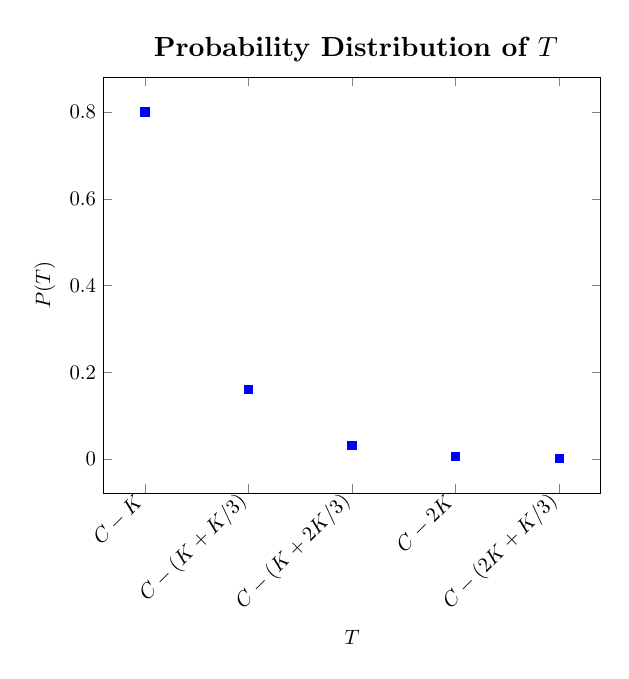
\begin{tikzpicture}[scale=0.75]
	\begin{axis}
	[% 
	scatter/classes={%
		a={mark=square*,blue},%
		b={mark=triangle*,red},%
		c={mark=o,draw=black}},
		xlabel={$T$},
		ylabel={$P(T)$},
		xtick={0, 1, 2, 3, 4},
		xticklabels={$C-K$, $C - (K + K/3)$, $C - (K + 2K/3)$, $C - 2K$, $C - (2K + K/3)$},x tick label style={rotate=45,anchor=east}],
		ytick={0.25, 0.5, 0.75, 1},
		ymax=1]
	\addplot[scatter,only marks,%
		scatter src=explicit symbolic]%
	table[meta=label] {
x     y      label
0      0.8   a     
1	0.16  a
2      0.032   a     
3      0.0064   a
4      0.00128   a   	  
	};
	\end{axis}
		\node[align=center,font=\bfseries, xshift=1.5em, yshift=1em] (title) 
    at (current bounding box.north)
    {Probability Distribution of $T$};
\end{tikzpicture}
\end{center}

%Question 4.7
\item  \begin{tcolorbox}[
  colback=Cerulean!5!white,
  colframe=Cerulean!75!black]
\textbf{Evaluate $\bm{P(X = 5)}$, where $\bm{X}$ is the random variable defined in Example 4.10. Suppose that $\bm{n_1 = 10}$, $\bm{n_2 = 15}$, $\bm{p_1 = 0.3}$, and $\bm{p_2 = 0.2}$.}
\end{tcolorbox}

Example 4.10 describes a situation in which there is a machine that, in the first $n_1$ attempts at operating it, there is a constant probability $p_1$ of making no error, and then in the following $n_2$ operation attempts, there is a constant probability of $p_2$ of making no error. The objective is to find the total number of successful operations of the machine across the $n_1 + n_2 = n$ operations.

The set up is as follows: let $X = k$ be the number of correct operations. Let $Y_1 = r$ and $Y_2 = k - r$ be the correct operations accomplished in the $n_1$ and $n_2$ attempts, respectively. Observe that for any $k$ and $r$, and if $S_1, S_2$ are successful operations in the $n_1$ and $n_2$ attempts, the successive attempts will look like

\[ \underbrace{ \underbrace{S_1 S_1 \cdots S_1}_{r} \underbrace{ \bar{S_1} \bar{S_1} \cdots \bar{S_1} }_{n_1 - r} }_{n_1} \underbrace{ \underbrace{S_2 S_2 \cdots S_2}_{k-r} \underbrace{ \bar{S_2} \bar{S_2} \cdots \bar{S_2} }_{n_2 - (k - r)} }_{n_2} \]

For some fixed $r,k$, we can see that there are $\binom{n_1}{r}$ ways of $r$ successes appearing out of $n_1$ attempts, and correspondingly, $\binom{n_2}{k-r}$ ways of $k-r$ success out of $n_2$ attempts. The probability $P(Y_1 = r)$ is then $\binom{n_1}{r} p_1^r (1-p_1)^{n_1 - r}$, and $P(Y_2 = k-r)$ is $\binom{n_2}{k - r} p_2^{k-r} (1 - p_2)^{n_2 - (k - r)}$; note that \textit{within} each of the $n_1, n_2$ attempts the probabilities of success or failure are constant and independent, which allows us to derive these equations. Now, because $Y_1$ and $Y_2$ are \textit{themselves} independent, to find the probability of $r$ successful operations in $n_1$ attempts \textit{and} $k-r$ successful operations in $n_2$ attempts is equivalent to writing

\[ P(X = k, Y_1 = r, Y_2 = k - r)=  \binom{n_1}{r} p_1^r (1-p_1)^{n_1 - r} \binom{n_2}{k - r} p_2^{k-r} (1 - p_2)^{n_2 - (k - r)} \]

However, the desired probability is to find $P(X = k)$. Applying the law of total probability for \textit{all} values of $r$ (since the events $Y_1 = r_1, Y_1 = r_2, ...$ are mutually exclusive) gives us

\[ P(X = k) = \sum^{n_1}_{r = 0} \binom{n_1}{r} p_1^r (1-p_1)^{n_1 - r} \binom{n_2}{k - r} p_2^{k-r} (1 - p_2)^{n_2 - (k - r)}  \] 

For the given values $k = 5, n_1 = 10, n_2 = 15, p_1 = 0.3, p_2 = 0.2$, we calculate

\[ P(X = 5) = \sum^{10}_{r = 0} \binom{10}{r} (0.3)^r (0.7)^{10 - r} \binom{15}{5 - r} (0.2)^{5-r} (0.8)^{(20 + r)} = \boxed{0.0189} \]

%Question 4.8
\item  \begin{tcolorbox}[
  colback=Cerulean!5!white,
  colframe=Cerulean!75!black]
\textbf{(\textit{Properties of the binomial probabilities.}) In the discussion of Example 4.8 a general pattern for the binomial probabilities $\binom{n}{k} \bm{p^k (1-p)^{n-k}}$ was suggested. Let us denote these probabilities by $\bm{p_n (k)}$.}
\end{tcolorbox}

	\begin{enumerate}
	%Question 4.8(a)
	\item  \begin{tcolorbox}[
	  colback=Cerulean!5!white,
	  colframe=Cerulean!75!black]
	\textbf{Show that for $\bm{0 \leq k < n}$ we have $\bm{p_n (k+1) / p_n (k) = [(n-k) / (k+1)] [p / (1 - p)]}$}
	\end{tcolorbox}
	
	\begin{proof}
	We have $p_n (k + 1) = \binom{n}{k+1} p^{k+1} (1-p)^{n-(k+1)} = \frac{n!}{(k+1)! (n- (k+1))!} p^{k+1} (1-p)^{n-(k+1)}$ and $p_n (k) = \binom{n}{k} p^k (1-p)^{n-k} = \frac{n!}{k! (n-k)!}  p^k (1-p)^{n-k}$. It immediately follows that $p_n (k+1) / p_n (k) = [(n-k) / (k+1)] [p / (1 - p)]$.
	\end{proof}
	
	%Question 4.8(b)
	\item  \begin{tcolorbox}[
	  colback=Cerulean!5!white,
	  colframe=Cerulean!75!black]
	\textbf{Using (a) show that}
	\end{tcolorbox}
	
		\begin{enumerate}
		%Question 4.8(b)(i)
		\item  \begin{tcolorbox}[
	  	colback=Cerulean!5!white,
	  	colframe=Cerulean!75!black]
		\textbf{$\bm{p_n (k + 1) > p_n (k)}$ if $\bm{k < np - (1 - p)}$,}
		\end{tcolorbox}
		
		\begin{proof}
		Equivalently, we demonstrate that $p_n (k+1) / p_n (k) > 1$. Suppose $k < np - (1 - p)$. Then $n - k > n - np + (1-p) = (1 - p)(n + 1)$ and $k + 1 < np - (1 - p) + 1 = p(n+1)$. Then $\frac{n-k}{k+1} > \frac{(1-p)(n+1)}{p(n+1)} = \frac{1-p}{p}$, implying $p_n (k+1) / p_n (k) = \frac{n-k}{k+1} \frac{p}{1-p} > \frac{1-p}{p} \frac{p}{1-p} = 1$.
		\end{proof}
		
		%Question 4.8(b)(ii)
		\item  \begin{tcolorbox}[
	  	colback=Cerulean!5!white,
	  	colframe=Cerulean!75!black]
		\textbf{$\bm{p_n (k + 1) = p_n (k)}$ if $\bm{k = np - (1 - p)}$,}
		\end{tcolorbox}
		
		\begin{proof}
		Equivalently, we demonstrate that $p_n (k+1) / p_n (k) = 1$. Suppose $k = np - (1 - p)$. Then $n - k = n - np + (1-p) = (1 - p)(n + 1)$ and $k + 1 = np - (1 - p) + 1 = p(n+1)$. Then $\frac{n-k}{k+1} = \frac{(1-p)(n+1)}{p(n+1)} = \frac{1-p}{p}$, implying $p_n (k+1) / p_n (k) = \frac{n-k}{k+1} \frac{p}{1-p} = \frac{1-p}{p} \frac{p}{1-p} = 1$.
		\end{proof}
		
			%Question 4.8(b)(iii)
		\item  \begin{tcolorbox}[
	  	colback=Cerulean!5!white,
	  	colframe=Cerulean!75!black]
		\textbf{$\bm{p_n (k + 1) < p_n (k)}$ if $\bm{k > np - (1 - p)}$.}
		\end{tcolorbox}
		
		\begin{proof}
		Equivalently, we demonstrate that $p_n (k+1) / p_n (k) < 1$. Suppose $k > np - (1 - p)$. Then $n - k < n - np + (1-p) = (1 - p)(n + 1)$ and $k + 1 > np - (1 - p) + 1 = p(n+1)$. Then $\frac{n-k}{k+1} < \frac{(1-p)(n+1)}{p(n+1)} = \frac{1-p}{p}$, implying $p_n (k+1) / p_n (k) = \frac{n-k}{k+1} \frac{p}{1-p} < \frac{1-p}{p} \frac{p}{1-p} = 1$.
		\end{proof}
		\end{enumerate}
		
	%Question 4.8(c)
	\item  \begin{tcolorbox}[
	  colback=Cerulean!5!white,
	  colframe=Cerulean!75!black]
	\textbf{Show that if $\bm{np - (1 - p)}$ is an integer, $\bm{p_n (k)}$ assumes its maximum value for two values of $\bm{k}$, namely $\bm{k_0 = np - (1 - p)}$ and $\bm{k'_0 = np - (1 - p) + 1}$.}
	\end{tcolorbox}
	
	\begin{proof}
	By (b)(ii), if $k_0 = np - (1-p)$, then $p_n (k_0) = p_n (k_0 + 1) = p_n (k'_0)$, the last equality from the fact that $k_0 + 1 = k'_0 = np - (1-p) + 1$. By (b)(i), $k_0 - 1 < k_0 \implies p_n(k_0) > p_n(k_0 - 1)$; ``induce downwards" to ascertain that decreasing $k_0 - 1, k_0 - 2,...$ implies that $p_n (k_0 - 1) > p_n (k_0 - 2) > \cdots$. Analogously, by (b)(iii), $k'_0 > k_0 \implies p_n(k'_0 + 1) < p_n(k'_0)$; ``induce upwards" to likewise ascertain that increasing $k'_0 + 1, k'_0 + 2, ...$ implies $p_n (k'_0 + 1) > p_n(k'_0 + 2) > \cdots$. Therefore, since values of $k$ moving away from $k_0, k'_0$ on either side cause $p_n$ to monotonically decrease, it follows that $k_0, k'_0$ are the maxima for $p_n$. \\
	
	Intuitively, this tells us that if $k_0 = np - (1-p)$ is an integer, then the binomial distribution will have \textit{two} modes differing by one.
	\end{proof}
	
	%Question 4.8(d)
	\item  \begin{tcolorbox}[
	  colback=Cerulean!5!white,
	  colframe=Cerulean!75!black]
	\textbf{Show that if $\bm{np - (1 - p)}$ is not an integer, $\bm{p_n (k)}$ assumes its maximum value when $\bm{k}$ is equal to the smallest integer greater than $\bm{k_0}$.}
	\end{tcolorbox}
	
	\begin{proof}\textbf{Strategy:} Define the \textbf{ceiling} $\lceil a \rceil$ of a real number $a$ as the smallest integer greater than $a$. If $k_0 = np - (1-p) \notin \mathbb{Z}$, then define $\lceil k_0 \rceil - k_0 = r$, for some $r, 0 < r < 1$; therefore, $\lceil k_0 \rceil = np - (1-p) + r$. The task before us is to evaluate if $p_n (\lceil k_o \rceil) > p_n (\lceil k_o \rceil - 1)$ and $p_n (\lceil k_o \rceil) > p_n (\lceil k_o \rceil + 1)$, or equivalently, if $\frac{p_n (\lceil k_o \rceil)}{p_n (\lceil k_o \rceil - 1)} > 1$ and $\frac{p_n (\lceil k_o \rceil + 1)}{p_n (\lceil k_o \rceil) } < 1$. Should we ascertain these conditions, then we may apply the monotonicity results of part (b) and conclude that $k = \lceil k_o \rceil$ is the (singular) maximum of of $p_n(k)$.
	
	First we consider the left-flank of $\lceil k_o \rceil$:
	
	\begin{align*}
	\frac{p_n (\lceil k_o \rceil)}{p_n (\lceil k_o \rceil - 1)} &= \frac{n - \lceil k_0 \rceil + 1}{\lceil k_0 \rceil} \frac{p}{1-p} \\
	&= \frac{n - ( np - (1-p) + r ) + 1}{np - (1-p) + r} \frac{p}{1-p} \\
	&= \frac{(1-p)(n+1) + (1-r)}{p(n+1) - (1-r)} \frac{p}{1-p} \\
	&> \frac{(1-p)(n+1)}{p(n+1)} \frac{p}{1-p} = 1
	\end{align*}
	
	And now the right-flank:
	
	\begin{align*}
	\frac{p_n (\lceil k_o \rceil + 1)}{p_n (\lceil k_o \rceil)} &= \frac{n - \lceil k_0 \rceil}{\lceil k_0 \rceil - 1} \frac{p}{1-p} \\
	&= \frac{n - (np - (1-p) + r)}{np - (1-p) + r + 1} \frac{p}{1-p} \\
	&= \frac{n (1-p) + (1-p) - r}{p(n+1) + r} \frac{p}{1-p} \\
	&< \frac{(1-p)(n+1)}{p(n+1)} \frac{p}{1-p} = 1
	\end{align*}
	
	In general, it can be shown that for any integer $i$, $0 \leq i \leq \lceil k_0 \rceil$, it is true that $\frac{p_n (\lceil k_o \rceil - i)}{p_n (\lceil k_o \rceil - (i+1))} > 1$, and analogously, $\frac{p_n (\lceil k_o \rceil + (j + 1))}{p_n (\lceil k_o \rceil + j)} < 1$ for any integer $j$, $0 \leq j \leq n - \lceil k_0 \rceil - 1$. Therefore, $p_n (\lceil k_0 \rceil)$ is the singular maximum.
	
	\end{proof}
	
	%Question 4.8(e)
	\item  \begin{tcolorbox}[
	  colback=Cerulean!5!white,
	  colframe=Cerulean!75!black]
	\textbf{Show that if $\bm{np - (1 - p) < 0}$, $\bm{p_n(0) > p_n(1) > \cdots > p_n(n)}$ while if $\bm{np - (1-p) = 0, p_n(0) = p_n(1) > p_n(2) > \cdots > p_n(n)}$.}
	\end{tcolorbox}
	
	\begin{proof}
	In the first case, apply (b)(iii) and since $k \geq 0 > np - (1-p)$, for $k = 0$ we have $p_n(0) > p_n(1)$, for $k=1$, $p_n(1) > p_n(2)$, and so-on-and-so-forth until $k = n-1$, $p_n (n-1) > p_n(n)$, establishing the result. In the second case, apply (b)(ii) for $k = np - (1-p) = 0$, therefore $p_n (0) = p_n(1)$, and for $k > np - (1-p) = 0$, apply (b)(iii) to get the desired result.
	\end{proof}

	\end{enumerate}

%Question 4.9
\item  \begin{tcolorbox}[
  colback=Cerulean!5!white,
  colframe=Cerulean!75!black]
\textbf{The continuous random variable $\bm{X}$ has pdf $\bm{f(x) = x/2, 0 \leq x \leq 2}$. Two independent determinations of $\bm{X}$ are made. What is the probability that both these determinations will be greater than one? If three independent determinations had been made, what is the probability that exactly two of these are larger than one?}
\end{tcolorbox}

In one determination, $P(1 < X) = \int^2_1 \frac{x}{2}dx = \frac{x^2}{4} \Big|^2_1 = 3/4$. By premise, each determination is independent, so we need only calculate $P(1 < X) P(1 < X) = \boxed{9/16}$. For the second case, there are $\binom{3}{2}$ ways in which exactly two of the three determinations are larger than one. The probability of one such scenario is $P(1 < X) P(1 < X) P(X \leq 1) = (3/4)^2 \cdot \int^1_0 \frac{x}{2}dx = (3/4)^2 1/4 = 9/64$. Multiply by $\binom{3}{2} = 3$ to get $\boxed{27/64}$. 

%Question 4.10
\item  \begin{tcolorbox}[
  colback=Cerulean!5!white,
  colframe=Cerulean!75!black]
\textbf{Let $\bm{X}$ be the life length of an electron tube and suppose that $\bm{X}$ may be represented as a continuous random variable with pdf $\bm{f(x) = be^{-bx}}$, $\bm{x \geq 0}$. Let $\bm{p_j} = P(j \leq X < j + 1)$. Show that $\bm{p_j}$ is of the form $\bm{(1-a)a^j}$ and determine $\bm{a}$.}
\end{tcolorbox}

Given the probability distribution function, we derive

\begin{align*}
\int^{j+1}_{j} be^{-bx} dx &= -e^{-bx} \Big|^{j+1}_j \\
&= -e^{-(j+1)x} + e^{-jx} \\
&= e^{-jx} (1 - e^{-x} ) \\
\end{align*}

Let $a = e^{-x}$, then the above becomes $(1-a)a^j$.

%Question 4.11
\item  \begin{tcolorbox}[
  colback=Cerulean!5!white,
  colframe=Cerulean!75!black]
\textbf{The continuous random variable $\bm{X}$ has pdf $\bm{f(x) = 3x^2, -1 \leq x \leq 0}$. If $\bm{b}$ is a number satisfying $\bm{-1 < b < 0}$, compute $\bm{P(X > b | X < b/2)}$.}
\end{tcolorbox}

By definition of conditional probability,

\begin{align*}
P(X > b | X < b/2) &= \frac{P(b < X < b/2)}{P(X < b/2)} \\
&= \frac{\int^{b/2}_b 3x^2 dx}{\int^{b/2}_{-1} 3x^2 dx} \\
&= \frac{x^3 \Big|^{b/2}_b}{x^3 \Big|^{b/2}_{-1}} \\
&= \frac{b^3/8 - b^3}{b^3/8 + 1} \\
&= \boxed{ \frac{-7b^3}{b^3 + 8} }
\end{align*}

%Question 4.12
\item  \begin{tcolorbox}[
  colback=Cerulean!5!white,
  colframe=Cerulean!75!black]
\textbf{Suppose that $\bm{f}$ and $\bm{g}$ are pdf's on the same interval, say $\bm{a \leq x \leq b}$.}
\end{tcolorbox}

	\begin{enumerate}
	%Question 4.12(a)
	\item  \begin{tcolorbox}[
	  colback=Cerulean!5!white,
	  colframe=Cerulean!75!black]
	\textbf{Show that $\bm{f + g}$ is not a pdf on that interval.}
	\end{tcolorbox}
	
	(Note: $\int$ shall mean $\int^{+\infty}_{-\infty}$)
	
	\begin{proof}
	By premise, $\int f(x) dx = 1$ and $\int g(x) dx = 1$. Then $\int f(x) dx + \int g(x) dx = \int (f(x) + g(x))dx = 2$, contradicting the definition of a probability distribution function. 
	\end{proof}
	
	%Question 4.12(b)
	\item  \begin{tcolorbox}[
	  colback=Cerulean!5!white,
	  colframe=Cerulean!75!black]
	\textbf{Show that for every number $\bm{\beta}$, $\bm{0 < \beta < 1, \beta f(x) + (1- \beta)g(x)}$ is a pdf on that interval.}
	\end{tcolorbox}
	
	\begin{proof}
	(1) By premise, $f(x), g(x) \geq 0$. Then $\beta f(x), (1 - \beta)g(x) \geq 0$ since $0 < \beta < 1$. \\
	(2) \begin{align*}
	\int ( \beta f(x) + (1- \beta)g(x) ) dx &= \int \beta f(x) dx + \int (1 - \beta) g(x) dx \\
	&= \beta \int f(x) dx + (1 - \beta) \int g(x) dx \\
	&= \beta + 1 - \beta = 1
	\end{align*}
	(3) By premise, $\int^b_a f(x) dx$ and $\int^b_a g(x) dx$ exist. For any $(a,b), a, b \in (-\infty, + \infty)$, it follows that
	\begin{align*}
	\beta \int^b_a  f(x) dx + (1 - \beta) \int^b_a  g(x) dx &= \int^b_a \beta f(x) dx + \int^b_a (1-\beta) g(x) dx \\
	&= \int^b_a ( \beta f(x) + (1- \beta)g(x) ) dx
	\end{align*}
	\end{proof}
	
	\end{enumerate}

%Question 4.13
\item  \begin{tcolorbox}[
  colback=Cerulean!5!white,
  colframe=Cerulean!75!black]
\textbf{Suppose that the graph in Fig. 4.16 represents the pdf of a random variable $\bm{X}$.}
\end{tcolorbox}

\begin{center}
	\begin{tikzpicture}[scale=0.75]
	\begin{axis}[
    	axis lines = center,
		ymax=7,
		ymin=0,
		xmin=-10,
		xmax=10,
   		 xlabel = \( x \),
   		 ylabel = {\( f(x) \)},
		 xtick={-8,0,6},
    		 xticklabels={$x=-a$,$$,$x=b$},
		 ytick={},
		 yticklabels={},
		]
	\addplot[domain=-8:4, style=very thick, color=red]{0.5*x+4};
	\addplot[domain=4:6, style=very thick, color=red]{-3*x+18};
	\node[draw] at (150,650) {$(a,b)$};
	\end{axis}
	\end{tikzpicture}
	\end{center}

	\begin{enumerate}
	%Question 4.13(a)
	\item  \begin{tcolorbox}[
	  colback=Cerulean!5!white,
	  colframe=Cerulean!75!black]
	\textbf{What is the relationship between $\bm{a}$ and $\bm{b}$?}
	\end{tcolorbox}
	
	The pdf is defined as
	
	\[f(x) = \begin{cases}
  \frac{b}{2a}x + \frac{b}{2},  &  -a \leq x < a \\
  \frac{b}{a-b} x - \frac{b^2}{a - b}, & a \leq x \leq b
\end{cases} \]

	Then it must be shown that the relationship between $a$ and $b$ is such that 
	
	\[ \int^a_{-a} \bigg( \frac{b}{2a} x + \frac{b}{2} \bigg) dx + \int^b_a \bigg( \bigg( \frac{b}{a-b} \bigg) x - \frac{b}{a-b} \bigg) dx = 1 \]
	
	With some algebra, it follows that $\boxed{a = (2/b) - b}$.
	
	%Question 4.13(b)
	\item  \begin{tcolorbox}[
	  colback=Cerulean!5!white,
	  colframe=Cerulean!75!black]
	\textbf{If $\bm{a > 0}$ and $\bm{b > 0}$, what can you say about the largest value which $\bm{b}$ may assume?}
	\end{tcolorbox}
	
	Fixing these constraints, we must have $0 < (2/b) - b \implies b^2 < 2 \implies \boxed{b < \sqrt{2}}$.
	\end{enumerate}
	
%Question 4.14
\item  \begin{tcolorbox}[
  colback=Cerulean!5!white,
  colframe=Cerulean!75!black]
\textbf{The percentage of alcohol $\bm{(100X)}$ in a certain compound may be considered as a random variable, where $\bm{X, 0 < X < 1}$, has the following pdf: $\bm{f(x) = 20 x^3 (1-x), 0 < x < 1}$}
\end{tcolorbox}

	\begin{enumerate}
	%Question 4.14(a)
	\item  \begin{tcolorbox}[
	  colback=Cerulean!5!white,
	  colframe=Cerulean!75!black]
	\textbf{Obtain an expression for the cdf $\bm{F}$ and sketch its graph.}
	\end{tcolorbox}
	
	By definition of cumulative distribution function, $F(x) = \int^x_0 20x^3 (1-x)dx = \boxed{5x^4 - 4x^5}$.
	
	\begin{center}
	\begin{tikzpicture}[scale=0.75]
	\begin{axis}[
    		axis lines = left,
		ymax=1,
		ymin=0,
   		 xlabel = \( X \),
   		 ylabel = {\( F(x) \)},
		 xtick={0,1},
    		 xticklabels={$0$,$1$},
		 ytick={0,1,1.5},
		 yticklabels={$0$,$1$,$$},
		]
	\addplot[domain=0:1, style=very thick, color=red]{5*x^4 - 4*x^5};
	\addplot[domain=1:1.5, style=very thick, color=red]{1};
	\end{axis}
	\end{tikzpicture}
	\end{center}
	
	%Question 4.14(b)
	\item  \begin{tcolorbox}[
	  colback=Cerulean!5!white,
	  colframe=Cerulean!75!black]
	\textbf{Evaluate $\bm{P(X \leq 2/3)}$.}
	\end{tcolorbox}
	
	$P(X \leq 2/3) = \int^{2/3}_0 = 20x^3 (1-x)dx = 5x^4 - 4x^5 \Big|^{2/3}_0 = \boxed{0.461}$
	
	%Question 4.14(c)
	\item  \begin{tcolorbox}[
	  colback=Cerulean!5!white,
	  colframe=Cerulean!75!black]
	\textbf{Suppose that the selling price of the above compound depends on the alcohol content. Specifically, if $\bm{1/3 < X < 2/3}$, the compound sells for $\bm{C_1}$ dollars/gallon; otherwise it sells for $\bm{C_2}$ dollars/gallon. If the cost is $\bm{C_3}$ dollars/gallon, find the probability distribution of the net profit per gallon.}
	\end{tcolorbox}
	
	$P(1/3 < X < 2/3) = \int^{2/3}_{1/3} 20x^3 (1-x)dx = 5x^4 - 4x^4 \Big|^{2/3}_{1/3} = \boxed{0.416}$
	
	Therefore, $P(\text{net profit is } C_1 - C_3) = \boxed{0.416}$ and $P(\text{net profit is } C_2 - C_3) = \boxed{0.584}$.
	\end{enumerate}

%Question 4.15
\item  \begin{tcolorbox}[
  colback=Cerulean!5!white,
  colframe=Cerulean!75!black]
\textbf{Let $\bm{X}$ be a continuous random variable with pdf $\bm{f}$ given by:}
\end{tcolorbox}

\[ f(x) = \begin{cases}
  ax  & 0 \leq x \leq 1 \\
  a & 1 \leq x \leq 2 \\
  -ax + 3a & 2 \leq x \leq 3 \\
  0 & \text{elsewhere}
\end{cases} \]

	\begin{enumerate}
	%Question 4.15(a)
	\item  \begin{tcolorbox}[
	  colback=Cerulean!5!white,
	  colframe=Cerulean!75!black]
	\textbf{Determine the constant $\bm{a}$.}
	\end{tcolorbox}
	
	By the Kolmogorov probability axioms, the definite integral of a pdf across the reals must be unity. Therefore, we must find a value of $a$ that acquiesces to this condition. We calculate:
	
	\begin{align*}
	&\int^1_0 ax dx + \int^2_1 adx + \int^3_2 (-ax + 3a)dx = 1 \\
	&\implies \frac{ax^2}{2} \Big|^1_0 + ax \Big|^2_1 + \Big( -\frac{ax^2}{2} + 3ax \Big) \Big|^3_2 = 1 \\
	&\implies \boxed{a = 1/2}
	\end{align*}
	
	%Question 4.15(b)
	\item  \begin{tcolorbox}[
	  colback=Cerulean!5!white,
	  colframe=Cerulean!75!black]
	\textbf{Determine $\bm{F}$, the cdf, and sketch its graph.}
	\end{tcolorbox}
	
	The cdf is defined as follows:
	
	$0 \leq X \leq 1: \int^x_0 \frac{1}{2}x dx = \frac{x^2}{4}$
	
	$1 \leq X \leq 2: \int^1_0 \frac{1}{2}x dx + \int^x_1 \frac{1}{2} dx = \frac{1}{4} + \frac{1}{2}x - \frac{1}{2}$
	
	$2 \leq X \leq 3: \int^1_0 \frac{1}{2}x dx + \int^2_1 \frac{1}{2} dx + \int^x_2 (-\frac{1}{2} x + \frac{3}{2} ) dx = \frac{1}{4} + 1 - \frac{1}{2} + ( -\frac{x^2}{4} + \frac{3}{2}x ) - 2$
	
	Therefore,
	
	\[ F(x) = \begin{cases}
  \frac{x^2}{4}  & 0 \leq X \leq 1 \\
  \frac{1}{2}x - \frac{1}{4} & 1 \leq X \leq 2 \\
  -\frac{x^2}{4} + \frac{3}{2}x - \frac{5}{4} & 2 \leq X \leq 3 \\
  1 & X \geq 3
\end{cases} \]

	\begin{center}
	\begin{tikzpicture}[scale=0.75]
	\begin{axis}[
    		axis lines = left,
		ymax=1,
		ymin=0,
   		 xlabel = \( X \),
   		 ylabel = {\( F(x) \)},
		 xtick={0,1,2,3},
    		 xticklabels={$0$,$1$,$2$,$3$},
		 ytick={0,1},
		 yticklabels={$0$,$1$},
		]
	\addplot[domain=0:1, color=red, style=very thick]{1/4*x^2};
	\addplot[domain=1:2, color=red, style=very thick]{1/2*x - 1/4};
	\addplot[domain=2:3, color=red, style=very thick]{-1/4*x^2 + 3/2*x - 5/4};
	\addplot[domain=3:3.5, color=red, style=very thick]{1};
	\end{axis}
	\end{tikzpicture}
	\end{center}
	
	%Question 4.15(c)
	\item  \begin{tcolorbox}[
	  colback=Cerulean!5!white,
	  colframe=Cerulean!75!black]
	\textbf{If $\bm{X_1, X_2,}$ and $\bm{X_3}$ are three independent observations from $\bm{X}$, what is the probability that exactly one of these three numbers is larger than 1.5?}
	\end{tcolorbox}
	
	Equivalently, one of the three independent observations is greater than 1.5 and the other two less than or equal to 1.5. There are $\binom{3}{1}$ such configurations. For any $X_i, P(X_i \leq 1.5) = (1/2)(3/2) - 1/4 = 1/2$. By complementary events, $P(X_i > 1.5) = 1/2$. Then we calculate $\binom{3}{1} (1/2)^3 = \boxed{3/8}$.
	\end{enumerate}
	
%Question 4.16
\item  \begin{tcolorbox}[
  colback=Cerulean!5!white,
  colframe=Cerulean!75!black]
\textbf{The diameter on an electric cable, say $\bm{X}$, is assumed to be a continuous random variable with pdf $\bm{f(x) = 6x(1-x), 0 \leq x \leq 1}$.}
\end{tcolorbox}

	\begin{enumerate}
	%Question 4.16(a)
	\item  \begin{tcolorbox}[
	  colback=Cerulean!5!white,
	  colframe=Cerulean!75!black]
	\textbf{Check that the above is a pdf and sketch it.}
	\end{tcolorbox}
	
	(1) For $0 \leq x \leq 1$, $x^2 \leq x$, so it follows that $6x - 6x^2 = 6x(1-x) \geq 0$ \\
	(2) $\int^1_0 6x(1-x) = 3x^2 - 2x^3 \Big|^1_0 = 1$ \\
	(3) $P(a \leq X \leq b) = \int^b_a 6x(1-x)dx$
	
	Therefore, $f(x)$ is a pdf.
	
	\begin{center}
	\begin{tikzpicture}[scale=0.75]
	\begin{axis}[
    		axis lines = left,
		ymax=1.5,
		ymin=0,
   		 xlabel = \( x \),
   		 ylabel = {\( f(x) \)},
		 xtick={0,1},
    		 xticklabels={$0$,$1$},
		 ytick={0,1},
		 yticklabels={$0$,$1$},
		]
	\addplot[domain=0:1, samples = 500, color=red, style=very thick]{6*x*(1-x)};
	\end{axis}
	\end{tikzpicture}
	\end{center}
	
	%Question 4.16(b)
	\item  \begin{tcolorbox}[
	  colback=Cerulean!5!white,
	  colframe=Cerulean!75!black]
	\textbf{Obtain an expression for the cdf of $\bm{X}$ and sketch it.}
	\end{tcolorbox}
	
	$F(x) = \int^x_0 6x(1-x)dx = \boxed{3x^2 - 2x^3}$
	
	\begin{center}
	\begin{tikzpicture}[scale=0.75]
	\begin{axis}[
    		axis lines = left,
		ymax=1,
		ymin=0,
   		 xlabel = \( x \),
   		 ylabel = {\( f(x) \)},
		 xtick={0,1},
    		 xticklabels={$0$,$1$},
		 ytick={0,1},
		 yticklabels={$0$,$1$},
		]
	\addplot[domain=0:1, samples = 500, color=red, style=very thick]{3*x^2 - 2*x^3};
	\end{axis}
	\end{tikzpicture}
	\end{center}
	
	%Question 4.16(c)
	\item  \begin{tcolorbox}[
	  colback=Cerulean!5!white,
	  colframe=Cerulean!75!black]
	\textbf{Determine a number $\bm{b}$ such that $\bm{P(X < b) = 2P(X > b)}$.}
	\end{tcolorbox}
	
	\begin{align*}
	&\int^b_0 6x(1-x)dx = 2 \int^1_b 6x(1-x)dx \\
	&\implies 3b^2 - 2b^3 = 2(1 - 3b^2 + 2b^3) \\
	&\implies -6b^3 + 9b^2 - 2 = 0 \\
	&\implies \boxed{b = 0.613}
	\end{align*}
	
	Note that there are two positive roots, but because our pdf is defined over $0 \leq X \leq 1$, we choose the one root within that domain.
	
	%Question 4.16(d)
	\item  \begin{tcolorbox}[
	  colback=Cerulean!5!white,
	  colframe=Cerulean!75!black]
	\textbf{Compute $\bm{P(X \leq 1/2 | 1/3 < X < 2/3)}$.}
	\end{tcolorbox}
	
	\begin{align*}
	P(X \leq 1/2 | 1/3 < X < 2/3) &= \frac{P(1/3 < X < 1/2)}{P(1/3 < X < 2/3)} \\
	&= \frac{\int^{1/2}_{1/3} 6x(1-x)dx}{\int^{2/3}_{1/3} 6x(1-x)dx} \\
	&= \boxed{0.5}
	\end{align*}
	
	\end{enumerate}

%Question 4.17
\item  \begin{tcolorbox}[
  colback=Cerulean!5!white,
  colframe=Cerulean!75!black]
\textbf{Each of the following functions represents the cdf of a continuous random variable. In each case $\bm{F(x) = 0}$ for $\bm{x < a}$ and $\bm{F(x) = 1}$ for $\bm{x > b}$, where $\bm{[a,b]}$ is the indicated interval. In each case, sketch the function $\bm{F}$, determine the pdf $\bm{f}$ and sketch it. Also verify that $\bm{f}$ is a pdf.}
\end{tcolorbox}

	\begin{enumerate}
	%Question 4.17(a)
	\item  \begin{tcolorbox}[
	  colback=Cerulean!5!white,
	  colframe=Cerulean!75!black]
	\textbf{$\bm{F(x) = x/5, 0 \leq x \leq 5}$}
	\end{tcolorbox}
	
	By Theorem 4.4, $\frac{d}{dx} F(x) = 1/5 = f(x)$. Clearly, $1/5 \geq 0 \ \forall x \in [0,5]$. Additionally, $\int^5_0 1/5 dx = x/5 \Big|^5_0 = 1$, and $\forall a, b$ such that $ [a, b] \subseteq [0, 5]$, we have $P(a \leq X \leq b) = \int^b_a 1/5 dx$. Therefore, $f(x) = 1/5$ is a pdf.
	
	\begin{center}
	\begin{tikzpicture}[scale=0.75]
	\begin{axis}[
    		axis lines = left,
   		 xlabel = \( x \),
   		 ylabel = {\( f(x) \)},
		 xtick={0,5},
    		 xticklabels={$0$,$5$},
		 ytick={0,1},
		 yticklabels={$0$,$1$},
		]
	\addplot[domain=0:5, samples = 500, color=red, style=very thick]{1/5};
	\end{axis}
	\end{tikzpicture}
	\end{center}
	
	%Question 4.17(b)
	\item  \begin{tcolorbox}[
	  colback=Cerulean!5!white,
	  colframe=Cerulean!75!black]
	\textbf{$\bm{F(x) = (2/ \pi) \arcsin (\sqrt{x}), 0 \leq x \leq 1}$}
	\end{tcolorbox}
	
	By Theorem 4.4, $\frac{d}{dx} F(x) = \frac{2}{\pi} \frac{1}{\sqrt{1-x}} \frac{1}{2} x^{-1/2} = \frac{1}{\pi} \frac{1}{\sqrt{x - x^2}} = f(x)$. Since $1/\pi \geq 0$ and $1/\sqrt{x - x^2} \geq 0 \ \forall x \in [0, 1]$, the product of the two terms must too be greater than or equal to 0. Additionally, $\int^1_0 \frac{1}{\pi} \frac{1}{\sqrt{x - x^2}} dx = (2/ \pi) \arcsin (\sqrt{x}) \Big|^1_0 = (2 / \pi) (\pi / 2) = 1$, and $P(a \leq X \leq b) = \int^b_a \frac{1}{\pi} \frac{1}{\sqrt{x - x^2}} dx \ \forall a, b$ such that $ [a, b] \subseteq [0, 1]$. Therefore, $f(x)$ is a pdf.
	
	\begin{center}
	\begin{tikzpicture}[scale=0.75]
	\begin{axis}[
    		axis lines = left,
   		 xlabel = \( x \),
   		 ylabel = {\( f(x) \)},
		 xtick={0,1},
    		 xticklabels={$0$,$1$},
		 ytick={0,1},
		 yticklabels={$0$,$1$},
		 trig format plots=rad,
		]
	\addplot[domain=0:1, samples = 500, color=red, style=very thick] {(2 / pi)*asin(sqrt(x)) };
	\end{axis}
	\end{tikzpicture}
	\end{center}
	
	%Question 4.17(c)
	\item  \begin{tcolorbox}[
	  colback=Cerulean!5!white,
	  colframe=Cerulean!75!black]
	\textbf{$\bm{F(x) = e^{3x}, -\infty < x \leq 0}$}
	\end{tcolorbox}
	
	By Theorem 4.4, $\frac{d}{dx} F(x) = 3e^{3x} = f(x)$. Since $e^{ax}$ for any $a$ is strictly positive, $f(x) \geq 0$ across the reals. Moreover, $\lim_{a \rightarrow -\infty} \int^0_a 3e^{3x} dx = \lim_{a \rightarrow -\infty} e^{3x} \big|^0_a = 1 - \lim_{a \rightarrow -\infty} e^{3a} = 1$, and $P(a \leq X \leq b) = \int^b_a 3e^{3x} dx \ \forall a, b$ such that $[a,b] \subseteq (-\infty, 0]$. Therefore, $f(x)$ is a pdf.
	
	\begin{center}
	\begin{tikzpicture}[scale=0.75]
	\begin{axis}[
    		axis lines = left,
   		 xlabel = \( x \),
   		 ylabel = {\( f(x) \)},
		xtick distance=1,
		]
	\addplot[domain=-5:0, samples = 500, color=red, style=very thick] { 3*exp(3*x) };
	\end{axis}
	\end{tikzpicture}
	\end{center}
	
	%Question 4.17(d)
	\item  \begin{tcolorbox}[
	  colback=Cerulean!5!white,
	  colframe=Cerulean!75!black]
	\textbf{$\bm{F(x) = x^3/2 + 1/2, -1 \leq x \leq 1}$}
	\end{tcolorbox}
	
	By Theorem 4.4, $\frac{d}{dx}F(x) = 3x^2 / 2 = f(x)$. Since $x^2 \geq 0 \ \forall x \in [-1, 1]$, it follows that $3x^2 / 2 + 1/2 \geq 0$ for that domain. Moreover, $P(-1 \leq X \leq 1) = F(1) - F(-1) = (1)^3/2 + 1/2 - ((-1)^3/2 + 1/2) = 1$, and $P(a \leq X \leq b) = F(b) - F(a) \ \forall a, b$ such that $[a,b] \subseteq [-1, 1]$. Therefore, $f(x)$ is a pdf.
	
	\begin{center}
	\begin{tikzpicture}[scale=0.75]
	\begin{axis}[
    		axis lines = left,
   		 xlabel = \( x \),
   		 ylabel = {\( f(x) \)},
		 xtick distance=1,
		 ytick distance=1,
		]
	\addplot[domain=-1:1, samples = 500, color=red, style=very thick] { 3*x^2/2 };
	\end{axis}
	\end{tikzpicture}
	\end{center}
	
	\end{enumerate}
	
%Question 4.18
\item  \begin{tcolorbox}[
  colback=Cerulean!5!white,
  colframe=Cerulean!75!black]
\textbf{Let $\bm{X}$ be the life length of an electronic device (measured in hours). Suppose that $\bm{X}$ is a continuous random variable with pdf $\bm{f(x) = k/x^n, 2000 \leq x \leq 10000}$.}
\end{tcolorbox}

	\begin{enumerate}
	%Question 4.18(a)
	\item  \begin{tcolorbox}[
	  colback=Cerulean!5!white,
	  colframe=Cerulean!75!black]
	\textbf{For $\bm{n = 2}$, determine $\bm{k}$.}
	\end{tcolorbox}
	
	By the Kolmogorov axioms, we must have $k$ such that $\int^{10000}_{2000} kx^{-2}dx = 1$.
	
	\begin{align*}
	\int^{10000}_{2000} kx^{-2}dx &= -kx^{-1} \big|^{10000}_{2000} \\
	&\implies k \Big( \frac{1}{2000} - \frac{1}{10000} \Big) = 1 \\
	&\implies \boxed{k = 2500}
	\end{align*}
	
	%Question 4.18(b)
	\item  \begin{tcolorbox}[
	  colback=Cerulean!5!white,
	  colframe=Cerulean!75!black]
	\textbf{For $\bm{n = 3}$, determine $\bm{k}$.}
	\end{tcolorbox}
	
	By the Kolmogorov axioms, we must have $k$ such that $\int^{10000}_{2000} kx^{-3}dx = 1$.

	\begin{align*}
	\int^{10000}_{2000} kx^{-3}dx &= -\frac{kx^{-2}}{2} \big|^{10000}_{2000} \\
	&\implies \frac{k}{2} \Big( \frac{1}{4 \cdot 10^6} - \frac{1}{10^8} \Big) = 1 \\
	&\implies \boxed{k = \frac{2.5 \cdot 10^7}{3}}
	\end{align*}
	
	%Question 4.18(c)
	\item  \begin{tcolorbox}[
	  colback=Cerulean!5!white,
	  colframe=Cerulean!75!black]
	\textbf{For general $\bm{n}$, determine $\bm{k}$.}
	\end{tcolorbox}
	
	For general $n$, we must have $k$ such that $\int^{10000}_{2000} kx^{-n}dx = 1$.
	
	\begin{align*}
	\int^{10000}_{2000} kx^{-n}dx &= -\frac{kx^{-(n-1)}}{n-1} \Big|^{10^4}_{2 \cdot 10^3} \\
	&\implies \frac{k}{n-1} \Bigg( \frac{1}{2^{n-1} 10^{3(n-1)} - \frac{1}{10^{4(n-1)}}} \Bigg) \\
	&\implies \boxed{ k = \frac{(n-1) 2^{n-1} \cdot 10^{4(n-1)}}{10^{n-1} - 2^{n-1}} }
	\end{align*}
	
	%Question 4.18(d)
	\item  \begin{tcolorbox}[
	  colback=Cerulean!5!white,
	  colframe=Cerulean!75!black]
	\textbf{What is the probability that the device will fail before 5000 hours have elapsed?}
	\end{tcolorbox}
	
	Using the previously calculated $k$ for $n=2$, we can calculate $\int^{5000}_{2000} kx^{-n} dx = -\frac{kx^{-(n-1)}}{n-1} \Big|^{5000}_{2000} = \boxed{0.75}$. Otherwise, calculate
	
	\begin{align*}
	\int^{5000}_{2000} kx^{-n} dx &= -\frac{kx^{-(n-1)}}{n-1} \Big|^{5000}_{2000} \\
	&= \frac{k}{n-1} \Bigg( \frac{1}{2000^{n-1}} - \frac{1}{5000^{n-1}} \Bigg) \\
	&= \boxed{ \frac{10^{n-1} - 4^{n-1} }{10^{n-1} - 2^{n-1}} }
	\end{align*}
	
	%Question 4.18(e)
	\item  \begin{tcolorbox}[
	  colback=Cerulean!5!white,
	  colframe=Cerulean!75!black]
	\textbf{Sketch the cdf $\bm{F(t)}$ for (c) and determine its algebraic form.}
	\end{tcolorbox}
	
	The cdf is derived by
	
	\begin{align*}
	\int^x_{2000} kx^{-n} dx &= -\frac{kx^{-(n-1)}}{n-1} \Big|^x_{2000} \\
	&= -\frac{kx^{-(n-1)}}{n-1} + \frac{k \cdot 2000^{-(n-1)}}{n-1} \\
	&= \frac{k}{n-1} \Bigg( \frac{1}{2000^{n-1} - \frac{1}{x^{n-1}}} \Bigg) \\
	&= \Bigg( \frac{2^{n-1} \cdot 10000^{n-1}}{10^{n-1} - 2^{n-1}} \Bigg) \Bigg( \frac{1}{2000^{n-1}} - \frac{1}{x^{n-1}} \Bigg) \\
	&= \frac{1}{10^{n-1} - 2^{n-1}} \Bigg( 10^{n-1} - \Bigg( \frac{20000}{x} \Bigg)^{n-1} \Bigg)
	\end{align*}
	
	For $n = 2$:
	
	\begin{center}
	\begin{tikzpicture}[scale=0.75]
	\begin{axis}[
    		axis lines = left,
		 ymax=1,
   		 xlabel = \( x \),
   		 ylabel = {\( F(x) \)},
		 xtick={2000,10000},
		 ytick distance=1,
		]
	\addplot[domain=2000:10000, samples = 100, color=red, style=very thick] { 1/8*(10 - 20000/x) };
	\end{axis}
	\end{tikzpicture}
	\end{center}
	\end{enumerate}

%Question 4.19
\item  \begin{tcolorbox}[
  colback=Cerulean!5!white,
  colframe=Cerulean!75!black]
\textbf{Let $\bm{X}$ be a binomially distributed random variable based on 10 repetitions of an experiment. If $\bm{p = 0.3}$, evaluate the following probabilities using the table of the binomial distribution in the Appendix.}
\end{tcolorbox}

Assume independence in successive repetitions.

	\begin{enumerate}
	%Question 4.19(a)
	\item  \begin{tcolorbox}[
	  colback=Cerulean!5!white,
	  colframe=Cerulean!75!black]
	\textbf{$\bm{P(X \leq 8)}$}
	\end{tcolorbox}
	
	Since $X$ may be 1 or 2 or $\cdots$ or 8, we calculate $P( X \leq 8) = \sum^8_{k = 1} \binom{10}{k} 0.3^k 0.7^{10-k} = \boxed{0.972}$.
	
	%Question 4.19(b)
	\item  \begin{tcolorbox}[
	  colback=Cerulean!5!white,
	  colframe=Cerulean!75!black]
	\textbf{$\bm{P(X = 7)}$}
	\end{tcolorbox}
	
	$P(X = 7) = \binom{10}{7} 0.3^7 0.7^3 = \boxed{0.009}$
	
	%Question 4.19(c)
	\item  \begin{tcolorbox}[
	  colback=Cerulean!5!white,
	  colframe=Cerulean!75!black]
	\textbf{$\bm{P(X > 6)}$}
	\end{tcolorbox}
	
	$P(X > 6) = \sum^10_{k = 7} \binom{10}{k} 0.3^k 0.7^{10-k} = \boxed{0.011}$
	\end{enumerate}
	
%Question 4.20
\item  \begin{tcolorbox}[
  colback=Cerulean!5!white,
  colframe=Cerulean!75!black]
\textbf{Suppose that $\bm{X}$ is uniformly distributed over $\bm{[-\alpha, +\alpha]}$, where $\bm{\alpha > 0}$. Whenever possible, determine $\bm{\alpha}$ so that the following are satisfied.}
\end{tcolorbox}

	By definition of uniform distribution, $f(x) = \frac{1}{\alpha - (-\alpha)} = 1/2\alpha$.

	\begin{enumerate}
	%Question 4.20(a)
	\item  \begin{tcolorbox}[
	  colback=Cerulean!5!white,
	  colframe=Cerulean!75!black]
	\textbf{$\bm{P(X > 1) = 1/3}$}
	\end{tcolorbox}
	
	\begin{align*}
	P(X > 1) &= \int^\alpha_1 \frac{1}{2\alpha} dx \\
	&= \frac{x}{2 \alpha} \Big|^\alpha_1 = \frac{\alpha}{2\alpha} - \frac{1}{2\alpha} = 1/3\\
	&\implies \boxed{\alpha = 3}
	\end{align*}
		
	%Question 4.20(b)
	\item  \begin{tcolorbox}[
	  colback=Cerulean!5!white,
	  colframe=Cerulean!75!black]
	\textbf{$\bm{P(X > 1) = 1/2}$}
	\end{tcolorbox}
	
	\begin{align*}
	P(X > 1) &= \int^\alpha_1 \frac{1}{2\alpha} dx \\
	&= \frac{x}{2 \alpha} \Big|^\alpha_1 = \frac{\alpha}{2\alpha} - \frac{1}{2\alpha} = 1/2\\
	&\implies \boxed{\text{No satisfactory value of }\alpha}
	\end{align*}
	
	%Question 4.20(c)
	\item  \begin{tcolorbox}[
	  colback=Cerulean!5!white,
	  colframe=Cerulean!75!black]
	\textbf{$\bm{P(X < 1/2) = 0.7}$}
	\end{tcolorbox}
	
	\begin{align*}
	P(X < 1/2) &= \int^{1/2}_{-\alpha} \frac{1}{2\alpha} dx \\
	&= \frac{x}{2\alpha} \Big|^{1/2}_{-\alpha} = \frac{1}{4\alpha} + \frac{1}{2} = 0.7 \\
	&\implies \boxed{\alpha = 5/4}
	\end{align*}
	
	%Question 4.20(d)
	\item  \begin{tcolorbox}[
	  colback=Cerulean!5!white,
	  colframe=Cerulean!75!black]
	\textbf{$\bm{P(X < 1/2) = 0.3}$}
	\end{tcolorbox}
	
	\begin{align*}
	P(X < 1/2) &= \int^{1/2}_{-\alpha} \frac{1}{2\alpha} dx \\
	&= \frac{x}{2\alpha} \Big|^{1/2}_{-\alpha} = 0.25 \frac{1}{\alpha} + 0.5 = 0.3 \\
	&\implies \boxed{\text{No satisfactory value of }\alpha}
	\end{align*}
	
	%Question 4.20(e)
	\item  \begin{tcolorbox}[
	  colback=Cerulean!5!white,
	  colframe=Cerulean!75!black]
	\textbf{$\bm{P(|X| < 1) = P(|X| > 1)}$}
	\end{tcolorbox}
	
	\begin{align*}
	\int^1_{-1} \frac{1}{2\alpha} dx &= \int^\alpha_1 \frac{1}{2\alpha} dx + \int^{-1}_{-\alpha} \frac{1}{2\alpha} dx \\
	\implies \frac{x}{2\alpha} \Big|^1_{-1} &= \frac{x}{2\alpha} \Big|^\alpha_1 + \frac{x}{2\alpha} \Big|^{-1}_{-\alpha} \\
	\implies \frac{1}{\alpha} &= \Bigg( \frac{1}{2} - \frac{1}{2\alpha} \Bigg) + \Bigg( -\frac{1}{2\alpha} + \frac{1}{2} \Bigg) \\
	\implies \boxed{\alpha = 2}
	\end{align*}
	
	\end{enumerate}
	
%Question 4.21
\item  \begin{tcolorbox}[
  colback=Cerulean!5!white,
  colframe=Cerulean!75!black]
\textbf{Suppose that $\bm{X}$ is uniformly distributed over $\bm{[0, \alpha]}$, $\bm{\alpha > 0}$. Answer the questions of Problem 4.20.}
\end{tcolorbox}

	By definition of uniform distribution, $f(x) = \frac{1}{\alpha}$.

	\begin{enumerate}
	%Question 4.21(a)
	\item  \begin{tcolorbox}[
	  colback=Cerulean!5!white,
	  colframe=Cerulean!75!black]
	\textbf{$\bm{P(X > 1) = 1/3}$}
	\end{tcolorbox}
	
	\begin{align*}
	P(X > 1) &= \int^\alpha_1 \frac{1}{\alpha} dx = \frac{1}{3} \\
	&= \frac{x}{\alpha} \Big|^\alpha_1 = 1 - \frac{1}{\alpha} = \frac{1}{3} \\
	&\implies \boxed{\alpha = 3/2}
	\end{align*}
	
	%Question 4.21(b)
	\item  \begin{tcolorbox}[
	  colback=Cerulean!5!white,
	  colframe=Cerulean!75!black]
	\textbf{$\bm{P(X > 1) = 1/2}$}
	\end{tcolorbox}
	
	\begin{align*}
	P(X > 1) &= \int^\alpha_1 \frac{1}{\alpha} dx = \frac{1}{2} \\
	&= \frac{x}{\alpha} \Big|^\alpha_1 = 1 - \frac{1}{\alpha} = \frac{1}{2} \\
	&\implies \boxed{\alpha = 2}
	\end{align*}
	
	%Question 4.21(c)
	\item  \begin{tcolorbox}[
	  colback=Cerulean!5!white,
	  colframe=Cerulean!75!black]
	\textbf{$\bm{P(X < 1/2) = 0.7}$}
	\end{tcolorbox}
	
	\begin{align*}
	P(X < 1/2) &= \int^{1/2}_{0} \frac{1}{\alpha} dx = 0.7 \\
	&= \frac{x}{\alpha} \Big|^{1/2}_{0} = \frac{1}{2\alpha} = 0.7 \\
	&\implies \boxed{\alpha = 5/7}
	\end{align*}
	
	%Question 4.21(d)
	\item  \begin{tcolorbox}[
	  colback=Cerulean!5!white,
	  colframe=Cerulean!75!black]
	\textbf{$\bm{P(X < 1/2) = 0.3}$}
	\end{tcolorbox}
	
	\begin{align*}
	P(X < 1/2) &= \int^{1/2}_{0} \frac{1}{\alpha} dx = 0.3 \\
	&= \frac{x}{\alpha} \Big|^{1/2}_{0} = \frac{1}{2\alpha} = 0.3 \\
	&\implies \boxed{\alpha = 5/3}
	\end{align*}
	
	%Question 4.21(e)
	\item  \begin{tcolorbox}[
	  colback=Cerulean!5!white,
	  colframe=Cerulean!75!black]
	\textbf{$\bm{P(|X| < 1) = P(|X| > 1)}$}
	\end{tcolorbox}
	
	\begin{align*}
	\int^1_0 \frac{1}{\alpha} dx &= \int^\alpha_1 \frac{1}{\alpha}dx \\
	\implies \frac{x}{\alpha} \Big|^1_0 &= \frac{x}{\alpha} \Big|^\alpha_1 \\
	\implies \frac{1}{\alpha} &= 1 - \frac{1}{\alpha} \\
	\implies \boxed{\alpha = 2}
	\end{align*}
	\end{enumerate}

%Question 4.22
\item  \begin{tcolorbox}[
  colback=Cerulean!5!white,
  colframe=Cerulean!75!black]
\textbf{A point is chosen at random on a line of length $\bm{L}$. What is the probability that the ratio of the shorter to the longer segment is less than 1/4?}
\end{tcolorbox}

Let $L$ be the length of the line. Suppose that the line is partitioned into two sections of length $x$ and $L-x$ such that $x < L-x$. Then the ratio of the short end to the long is $x / (L-x)$. The first objective is to determine a pdf $f(x)$ that satisfies the Kolmogorov axioms. To do so, suppose $f(x) = \alpha \frac{x}{L-x}$. Then we must find a value of $\alpha$ such that $\alpha \int^1_0 \frac{x}{L-x}dx = 1$. Integration by substitution, for $u = L-x$ and $du = -1 \cdot dx$, allows us to derive

\begin{align*}
\alpha \int^1_0 \frac{x}{L-x}dx &= \alpha [L - x - L \ln (L-x)] \Big|^1_0 = 1 \\
&= \alpha \Bigg[ -1 + \ln \Bigg( \Bigg( \frac{L}{L-1} \Bigg)^L \Bigg) \Bigg] = 1 \\
&\implies \boxed{\alpha = \frac{1}{\ln \Big( \Big( \frac{L}{L-1} \Big)^L \Big) - 1}}
\end{align*}

For $L > 1$, $\alpha > 0$. Since $x < L$, it follows that $x / (L-x) \geq 0$, and so $f(x) \geq 0$, thus satisfying the Kolmogorov axioms to be a pdf. Calculating the probability that the ratio of the short to long segment is less than $1/4$ gives us

\begin{align*}
P\Big( \frac{x}{L-x} < 1/4 \Big) &= \alpha \int^{1/4}_0 \frac{x}{L-x} dx \\
&= \alpha [L-x-L \ln (L-x)] \Big|^{1/4}_0 \\
&= \alpha \Big[ \ln \Big( \Big( \frac{L}{L - 1/4} \Big)^L \Big) - \frac{1}{4} \Big] \\
&= \boxed{ \frac{ \ln \Big( \Big( \frac{L}{L - 1/4} \Big)^L \Big) - \frac{1}{4} }{ \ln \Big( \Big( \frac{L}{L-1} \Big)^L \Big) - 1 } }
\end{align*}

%Question 4.23
\item  \begin{tcolorbox}[
  colback=Cerulean!5!white,
  colframe=Cerulean!75!black]
\textbf{A factory produces 10 glass containers daily. It may be assumed that there is a constant probability $\bm{p = 0.1}$ of producing a defective container. Before these containers are stored they are inspected and the defective ones are set aside. Suppose that there is a constant probability $\bm{r = 0.1}$ that a defective container is misclassified. Let $\bm{X}$ equal the number of containers classified as defective at the end of a production day. (Suppose that all containers which are manufactured on a particular day are also inspected on that day.)}
\end{tcolorbox}

	\begin{enumerate}
	%Question 4.23(a)
	\item  \begin{tcolorbox}[
	  colback=Cerulean!5!white,
	  colframe=Cerulean!75!black]
	\textbf{Compute $\bm{P(X = 3)}$ and $\bm{P(X > 3)}$.}
	\end{tcolorbox}
	
	%Question 4.23(b)
	\item  \begin{tcolorbox}[
	  colback=Cerulean!5!white,
	  colframe=Cerulean!75!black]
	\textbf{Obtain an expression for $\bm{P(X = k)}$.}
	\end{tcolorbox}
	\end{enumerate}

%Question 4.24
\item  \begin{tcolorbox}[
  colback=Cerulean!5!white,
  colframe=Cerulean!75!black]
\textbf{Suppose that 5 percent of all items coming off a production line are defective. If 10 such items are chosen and inspected, what is the probability that at most 2 defectives are found?}
\end{tcolorbox}

Equivalently, we find the probability that 0, 1, or 2 items are defective. In choosing 10 items with a 5 percent probability of defectiveness on the production line, we calculate $\sum^2_{i=0} \binom{10}{i} (0.05)^i (1-0.95)^{10-i} = \boxed{0.988}$.

%Question 4.25
\item  \begin{tcolorbox}[
  colback=Cerulean!5!white,
  colframe=Cerulean!75!black]
\textbf{Suppose that the life length (in hours) of a certain radio tube is a continuous random variables $\bm{X}$ with pdf $\bm{f(x) = 100/x^2, x > 100}$, and 0 elsewhere.}
\end{tcolorbox}

	\begin{enumerate}
	%Question 4.25(a)
	\item  \begin{tcolorbox}[
	  colback=Cerulean!5!white,
	  colframe=Cerulean!75!black]
	\textbf{What is the probability that a tube will last less than 200 hours if it is known that the tube is still functioning after 150 hours of service?}
	\end{tcolorbox}
	
	We find the probability that the tube lasts less than 200 hours conditional on the fact that it is still functioning after 150 hours, or $P(X < 200 | X > 150) = \frac{P(150 < X < 200)}{P(X > 150)} = \frac{\int^{200}_{150} \frac{100}{x^2} dx }{\int^{+\infty}_{150} \frac{100}{x^2} dx} = \boxed{1/4}$
	
	%Question 4.25(b)
	\item  \begin{tcolorbox}[
	  colback=Cerulean!5!white,
	  colframe=Cerulean!75!black]
	\textbf{What is the probability that if 3 such tubes are installed in a set, exactly one will have to be replaced after 150 hours of service?}
	\end{tcolorbox}
	
	Conceptually, if $A$ is the event that the a tube between 100 to 150 hours, then $\bar{A} = 1 - P(A)$ is the event it does not. Then $P(A) = \int^{150}_{100} \frac{100}{x^2}dx$ and we can calculate $\binom{3}{1} [\int^{150}_{100} \frac{100}{x^2} dx] [1 - \int^{150}_{100} \frac{100}{x^2} dx]^2 = \boxed{4/9}$.
	
	%Question 4.25(c)
	\item  \begin{tcolorbox}[
	  colback=Cerulean!5!white,
	  colframe=Cerulean!75!black]
	\textbf{What is the maximum number of tubes that may be inserted into a set so that there is a probability of 0.5 that after 150 hours of service all of them are still functioning?}
	\end{tcolorbox}
	
	Since each tube's lifespan is independent of one another, if $A$ is the event that a tube lasts longer than 150 hours, then we need only calculate the floor value of $n$, or $\floor{n}$ such that $P(A)^n = 0.5$. Thus we calculate $P(A) = \int^{+\infty}_{150} \frac{100}{x^2} dx = 2/3$. Then
	
	\begin{align*}
	P(A)^n &= (2/3)^n = 0.5 \\
	\implies n \ln (2/3) &= \ln (0.5) \\
	\implies n &= \frac{\ln (0.5)}{ \ln(2/3)}
	\end{align*}
	
	Therefore, $\boxed{\floor{n} = 1}$.
	
	\end{enumerate}

%Question 4.26
\item  \begin{tcolorbox}[
  colback=Cerulean!5!white,
  colframe=Cerulean!75!black]
\textbf{An experiment consists of $\bm{n}$ independent trials. It may be supposed that because of ``learning," the probability of obtaining a successful outcome increases with the number of trials performed. Specifically, suppose that $\bm{P}$(success on the ith repetition) $\bm{= (i+1)/(i+2), i = 1,2,...,n}$.}
\end{tcolorbox}

	\begin{enumerate}
	%Question 4.26(a)
	\item  \begin{tcolorbox}[
	  colback=Cerulean!5!white,
	  colframe=Cerulean!75!black]
	\textbf{What is the probability of having at least 3 successful outcomes in 8 repetitions?}
	\end{tcolorbox}
	
	Alternatively, consider 1 minus the sum of the probabilities of having 0, 1, and 2 successful outcomes in 8 repetitions. The probability of having zero successful outcomes in 8 repetitions is $\Pi_{i=1}^8 (1 - \frac{i+1}{i+2})$. To calculate for one and two, it is necessary to go through each of the configurations in which any one or any two of the eight repetitions are successful; because the probability of success of the $i$-th repetition differs as $i$ changes, this is tedious to calculate and is left to the reader.
	
	%Question 4.26(b)
	\item  \begin{tcolorbox}[
	  colback=Cerulean!5!white,
	  colframe=Cerulean!75!black]
	\textbf{What is the probability that the first successful outcome occurs on the eighth repetition?}
	\end{tcolorbox}
	
	If the probability of success on the $i$-th repetition is $P(i) = \frac{i+1}{i+2}$, then to not be successful on the $i$-th probability is $1 - \frac{i+1}{i+2}$. Assuming each repetition is independent of one another, then we can calculate $\Pi_{i=1}^7 (1 - \frac{i+1}{i+2}) (9/10) = \boxed{2.6 \cdot 10^{-6}}$.
	
	\end{enumerate}

%Question 4.27
\item  \begin{tcolorbox}[
  colback=Cerulean!5!white,
  colframe=Cerulean!75!black]
\textbf{Referring to Example 4.10,}
\end{tcolorbox}

	\begin{enumerate}
	%Question 4.27(a)
	\item  \begin{tcolorbox}[
	  colback=Cerulean!5!white,
	  colframe=Cerulean!75!black]
	\textbf{evaluate $\bm{P(X = 2)}$ if $\bm{n=4}$,}
	\end{tcolorbox}
	
	Suppose that $n_1, n_2 \neq 0$ (namely, we ensure that we have two non-empty sets of $n_1$ and $n_2$ repetitions). Further assume $p_1 = 0.2$ and $p_2 = 0.1$ as in Example 4.10. Then we can calculate $P(X = 2) = \sum^3_{n_1 = 1} [ \sum^{n_1}_{r=0} \binom{n_1}{r} p_1^r (1 - p_1)^{n_1 - r} \binom{4 - n_1}{2 - r} p_2^{2-r} (1 - p_2)^{4 - n_1 - (2-r)} ] = \boxed{0.2914}$.
	
	%Question 4.27(b)
	\item  \begin{tcolorbox}[
	  colback=Cerulean!5!white,
	  colframe=Cerulean!75!black]
	\textbf{for arbitrary $\bm{n}$, show that $\bm{P(X = n - 1) = P}$ (exactly one unsuccessful attempt) is equal to $\bm{[1 / (n+1)] \sum^n_{i=1} (1/i)}$.}
	\end{tcolorbox}
		
	\end{enumerate}

%Question 4.28
\item  \begin{tcolorbox}[
  colback=Cerulean!5!white,
  colframe=Cerulean!75!black]
\textbf{If the random variable $\bm{K}$ is uniformly distributed over $\bm{(0,5)}$, what is the probability that the roots of the equation $\bm{4x^2 + 4xK + K + 2 = 0}$ are real?}
\end{tcolorbox}

Firstly, by definition of uniform distribution, $f(x) = 1/5, 0 \leq x \leq 5$. By the quadratic equation, the roots of the second-degree polynomial $4x^2 + 4xK + K + 2 = 0$ are $\frac{-K \pm \sqrt{(K - 2) (K + 1)}}{2}$. The quantity under the radical is greater than or equal to $0$ only when $K \geq 2$ or $K \leq -1$. Therefore, we must calculate the probability $P(2 \leq X \leq 5)$, or $\int^5_2 1/5 dx = \boxed{3/5}$. 

%Question 4.29
\item  \begin{tcolorbox}[
  colback=Cerulean!5!white,
  colframe=Cerulean!75!black]
\textbf{Suppose that the random variable $\bm{X}$ has possible values 1, 2, 3, ... and that $\bm{P(X = r) = k(1 - \beta)^{r - 1}, 0 < \beta < 1}$.}
\end{tcolorbox}

	\begin{enumerate}
	%Question 4.29(a)
	\item  \begin{tcolorbox}[
	  colback=Cerulean!5!white,
	  colframe=Cerulean!75!black]
	\textbf{Determine the constant $\bm{k}$.}
	\end{tcolorbox}
	
	By the Kolmogorov axioms of probability, we must have $\sum^\infty_{i=1} P(X = i) = 1$. Equivalently, we must have $k [ 1 + (1 - \beta) + (1 - \beta)^2 + \cdots] = 1$. By premise, we can deduce that $|1 - \beta| < 1$; appealing to the closed-form expression of an infinite geometric series with common ratio strictly less than 1, we can deduce that the bracketed term simplifies to $1 \ \beta$; therefore $\boxed{k = \beta}$.
	
	%Question 4.29(b)
	\item  \begin{tcolorbox}[
	  colback=Cerulean!5!white,
	  colframe=Cerulean!75!black]
	\textbf{Find the mode of this distribution (i.e., that value of $\bm{r}$ which makes $\bm{P(X = r)}$ largest).}
	\end{tcolorbox}
	
	By inspection, $\beta (1 - \beta)^{r-1}$ is maximized when $\boxed{r = 1}$. This is apparent because $\beta > \beta(1 - \beta) > \beta(1 - \beta)^2 > \cdots$. 

	\end{enumerate}
	
%Question 4.30
\item  \begin{tcolorbox}[
  colback=Cerulean!5!white,
  colframe=Cerulean!75!black]
\textbf{A random variable $\bm{X}$ may assume four values with probabilities $\bm{(1 + 3x) / 4, (1-x)/4, (1+2x)/4}$, and $\bm{(1-4x) / 4}$. For what values of $\bm{x}$ is this a probability distribution?}
\end{tcolorbox}

Observe that the sum of the probabilities is 1 irrespective for any value of $x$. However, each of the individual probabilities must be bounded by $[0,1]$. The intersection of the intervals for which this is true will be the range of $x$ that satisfies the Kolmogorov probability axioms.

\begin{align*}
0 \leq \frac{1 + 3x}{4} \leq 1 &\implies -1/3 \leq x \leq 1 \\
0 \leq \frac{1 - x}{4} \leq 1 &\implies -3 \leq x \leq 1 \\
0 \leq \frac{1 + 2x}{4} \leq 1 &\implies -1/2 \leq x \leq 3/2 \\
0 \leq \frac{1 - 4x}{4} \leq 1 &\implies -3/4 \leq x \leq 1/4 \\
\end{align*}

The intersection of these intervals is $\boxed{-1/3 \leq x \leq 1/4}$.

\end{enumerate}

\end{document}  